\chapter{Teoría de las curvas elípticas}

\section{Introducción y motivación}
Los investigadores llevaban años buscando funciones más seguras para criptografía y en 1985 se propuso por primera vez el uso de curvas elípticas como base del problema del logaritmo discreto en un grupo~\cite{Koblitz1987,Miller1986}. Se cree que las curvas elípticas ofrecen un nivel de seguridad equivalente al de RSA pero con tamaños de clave mucho menores. Para ilustrar la diferencia en términos intuitivos, comparemos la energía necesaria para romper los diferentes sistemas con la cantidad de agua que esa energía podría hervir~\cite{Rickard2016,Lenstra2000}:
\begin{itemize}
  \item Romper una clave RSA de 228 bits requiere menos energía que la necesaria para hervir una cucharadita de agua.  
  \item Romper una clave ECC de 228 bits equivaldría a la energía necesaria para hervir toda el agua de la Tierra.  
  \item Para obtener el mismo nivel de seguridad con RSA haría falta una clave de unos 2 380 bits, lo cual es muy ineficiente en entornos con recursos limitados.  
\end{itemize}

Como hemos mencionado anteriormente en el capítulo~\ref{chap:Campos_finitos}, la eficiencia de los esquemas basados en curvas elípticas depende directamente de la velocidad de los algoritmos de aritmética de curva, que a su vez recaen en las operaciones sobre el campo (suma, multiplicación, inversión)...

La figura~\ref{fig:ECDSA_esquema} muestra las bases necesarias para entender e implementar un protocolo como el algoritmo de firma digital de curva elíptica (ECDSA). La aritmética de curvas no solo se construye sobre las operaciones en el campo subyacente, sino que en algunos casos también requiere aritmética de grandes enteros y operaciones modulares. ECDSA emplea una función hash y ciertas operaciones modulares, pero los pasos más costosos desde el punto de vista computacional son las propias operaciones en la curva.
\begin{figure}[H]
    \centering
    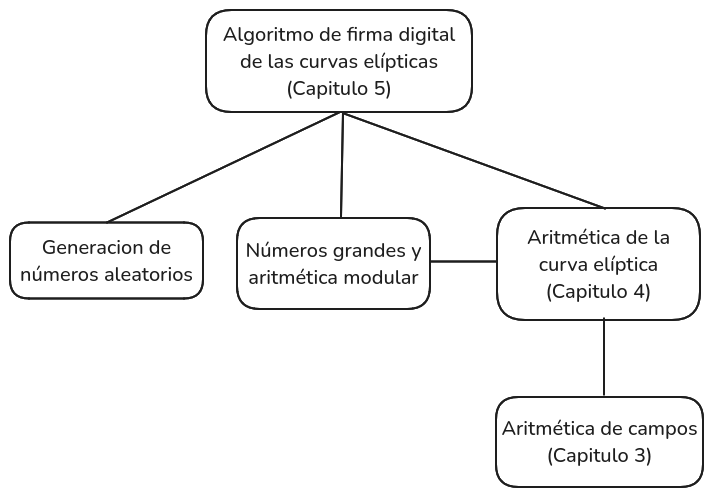
\includegraphics[width=0.8\textwidth]{imagenes/ECDSA_esquema.png}
    \caption{Esquema del Algoritmo de firma digital de las curvas elípticas (ECDSA)}
    \label{fig:ECDSA_esquema}
\end{figure}
%need to update this
La sección~\ref{sec:historia_curvas_elipticas} ofrece una introducción a las curvas elípticas donde se presentan las operaciones de grupo de suma y duplicado para los puntos de la curva, junto con su estructura fundamental y otras propiedades básicas. La sección~3.2 expone las representaciones en coordenadas proyectivas (y los algoritmos asociados de suma y duplicado), de especial interés cuando la inversión en el campo es más cara que la multiplicación. La sección~3.3 discute estrategias para la multiplicación de puntos.

Los métodos de las secciones~3.4, 3.5 y 3.6 están relacionados en que todos ellos explotan endomorfismos de la curva para reducir el coste del duplicado en la multiplicación de puntos. La sección~3.4 trata las curvas de Koblitz especiales, que permiten sustituir el duplicado de punto sobre \(\mathbb{F}_2\) por operaciones de cuadrado en el campo, mucho más baratas. La sección~3.5 examina una clase más amplia de curvas elípticas que admiten endomorfismos usados eficientemente para disminuir el número de duplicaciones. Las estrategias de la sección~3.6, para curvas sobre campos binarios, reemplazan la mayoría de los duplicados por una operación de “halving” de punto, potencialmente más rápida. La sección~3.7 recoge comparaciones de conteo de operaciones para métodos seleccionados de multiplicación de puntos. Finalmente, la sección~3.8 concluye con notas del capítulo y referencias.


\subsection{Historia y aplicaciones}\label{sec:historia_curvas_elipticas}
En 1997 Certicom lanzó el \emph{ECC Challenge} para evaluar la dificultad práctica del problema del logaritmo discreto en curvas elípticas, proponiendo instancias que hoy en día siguen siendo un referente en seguridad~\cite{gaudry2007breaking}. Pocos años después, en 1998, el comité ANSI X9 publicó la norma X9.62 definiendo el algoritmo de firma ECDSA, marcando el primer estándar formal para firmas basadas en curvas elípticas~\cite{ansi_x962_1998}. 
En el año 2000, el NIST incorporó curvas elípticas en el FIPS 186–2 (Digital Signature Standard), consolidando su uso en aplicaciones gubernamentales y financieras~\cite{nist_fips186_2}.

En 2005 la NSA anunció la Suite B de algoritmos criptográficos, recomendando las curvas P-256, P-384 y P-521 para uso en comunicaciones seguras de nivel gubernamental~\cite{rfc5430}. Con la adopción de TLS 1.2 y la publicación del RFC 8422 en 2018, las curvas secp256r1 (también conocida como prime256v1) y X25519 se convirtieron en cimientos de la seguridad de Internet, al ofrecer un excelente equilibrio entre rendimiento y seguridad~\cite{rfc8422}.

Los esquemas de intercambio de clave ECDH y de firma ECDSA aprovechan la elevada seguridad por bit de las curvas, permitiendo, por ejemplo, igualar la fuerza de una clave RSA de 3072 bits con una curva de solo 256 bits~\cite{hankerson2004guide}.
Protocolos tan extendidos como TLS (RFC 4492) o SSH (RFC 5656) incluyen suites para ECC, acelerando el establecimiento de sesiones seguras~\cite{rfc4492,rfc5656}. En sistemas distribuidos, Bitcoin emplea la curva secp256k1 para generar direcciones y validar transacciones, gracias a su código optimizado y su fortaleza criptográfica~\cite{wuille2017secp256k1}.

En entornos con recursos limitados, como dispositivos IoT o tarjetas inteligentes, ECC ha demostrado reducir consumo energético y acelerar operaciones criptográficas frente a RSA, al requerir menos ciclos de CPU y menos memoria~\cite{hodges2001implementing}. Además, las propiedades algebraicas de las curvas han sido la base para esquemas avanzados como sistemas de emparejamientos (pairing-based cryptography), identidades basadas en curva (IBE) y firmas Schnorr y EdDSA, ampliando enormemente el catálogo de construcciones criptográficas eficientes~\cite{boneh2001identity}.

\section{Definición de una curva elíptica}\label{sec:definicion_curvas_elipticas}
\subsection{Forma de Weierstrass general}\label{sec:weierstrass_curvas_elipticas}
\subsection{Transformaciones y cambios de coordenadas}

\section{Estructura de grupo}
\subsection{Punto en el infinito}
\subsection{Ley de suma de puntos (geometría proyectiva)}
\subsection{Propiedades algebraicas}

\section{Curvas sobre cuerpos finitos}\label{sec:curvas_sobre_cuerpos_finitos}
\subsection{Curvas sobre \texorpdfstring{$\mathbb{F}_p$}{Fp}}\label{sec:curvas_sobre_cuerpos_finitos_primos}
\subsection{Curvas binarias sobre \texorpdfstring{$\mathbb{F}_{2^m}$}{F2m}}\label{sec:curvas_sobre_cuerpos_finitos_binarios}

\section{Coordenadas y representación}\label{sec:coordenadas_curvas_elipticas}
\subsection{Coordenadas afines}
\subsection{Coordenadas proyectivas y Jacobianas}
\subsection{Coordenadas 'mixed' y optimizaciones}

\section{Selección de parámetros}
\subsection{Tamaños de curva y seguridad}
\subsection{Cofactores y subgrupos}
\subsection{Curvas estandarizadas (secp256k1, Curve25519, …)}